\documentclass[12pt]{article}
\usepackage{enumerate}
\usepackage{mathematics}
\usepackage{oxford}

\newcommand{\Ch}{\mathcal{C}_h}

\begin{document}
\title{Oxford M1 - Groups and Group Actions \footnotetext{\url{https://courses.maths.ox.ac.uk/node/5552}}}
\author{}
\date{}
\maketitle

\section{Sheet 1: Binary Operations. The Group Axioms. Examples.}

\begin{mdframed}
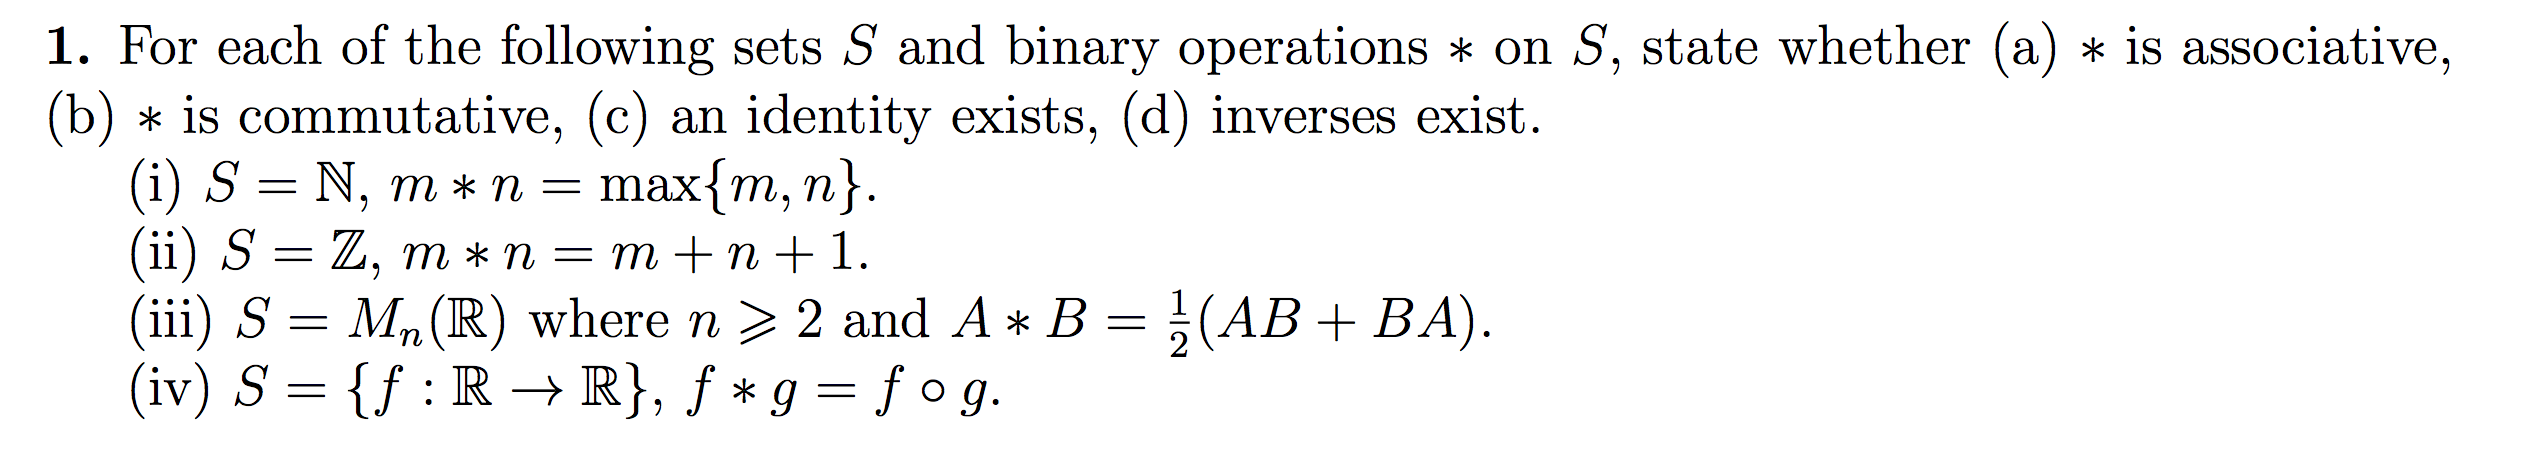
\includegraphics[width=400pt]{img/oxford-prelims-M1-groups-1-1.png}
\end{mdframed}
\begin{enumerate}[label=(\roman*)]
\item associative, commutative, identity is $e = 0$, only inverse is $e^\1 = e$.
\item associative, commutative, identity is $e = -1$, inverse is $m^\1 = -m - 2$.
\item \red{(not) associative?}, commutative, identity is $I_n$, inverse is $A^\1$\\
  Note that if $AB = BA$ then $A\cdot B = AB$, and $A\cdot(B\cdot C) = A(BC) = (AB)C$. I.e. the
  operation is associative for commutative matrices.\\

  Let $A$ be a reflection and $B$ a shear:
  $A = \matMMxNN{-1}{0}
                {0}{1}$, $B = \matMMxNN{1}{\frac{1}{\sqrt{2}}}
                                       {0}{\frac{1}{\sqrt{2}}}$.\\
  Then $AB = \matMMxNN{-1}{-\frac{1}{\sqrt{2}}}
                      {0}{~~\frac{1}{\sqrt{2}}}$ and
  and  $BA = \matMMxNN{-1}{\frac{1}{\sqrt{2}}}
                      {0}{\frac{1}{\sqrt{2}}}$,
  and $\frac{1}{2}(AB + BA) = \matMMxNN{-1}{0}
                                       {0}{\frac{1}{\sqrt{2}}}$.\\

  % E.g. let $A = I, B = 2I, C=3I$.\\
  % Then $A\cdot (B\cdot C) = I\cdot (6I)$ and $(A \cdot B)\cdot C) = 2I \cdot 3I = 6I$.
\item associative (function composition is associative), not commutative, identity is $I$, inverses
  only exist for bijections.
\end{enumerate}

\begin{mdframed}
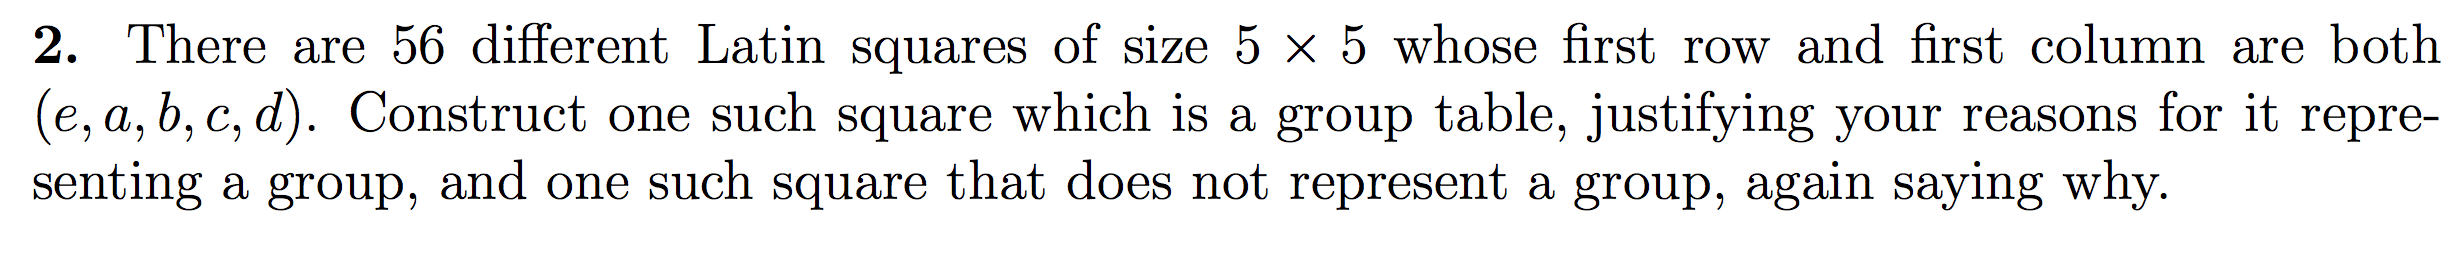
\includegraphics[width=400pt]{img/oxford-prelims-M1-groups-1-2.png}
\end{mdframed}
These both satisfy existence of identity and inverses because they are Latin squares.

Latin square, group:\\~\\
\begin{tabular}{c||c|c|c|c|c|}
    & e & a & b & c & d\\
  \hline
  \hline
  e & e & a & b & c & d\\
  a & a & b & c & d & e\\
  b & b & c & d & e & a\\
  c & c & d & e & a & b\\
  d & d & e & a & b & c
\end{tabular}\\
Group because it's isomorphic to $\Z/5\Z$.\\
Associative: e.g. $a(bc) = ae = a$ and $(ab)c = cc = a$.
Commutative.

~\\~\\
\red{Latin square, not a group:}\\~\\
\begin{tabular}{c||c|c|c|c|c|}
    & e & a & b & c & d\\
  \hline
  \hline
  e & e & a & b & c & d\\
  a & a &&&&\\
  b & b &&&&\\
  c & c &&&&\\
  d & d &&&&
\end{tabular}

\newpage
\begin{mdframed}
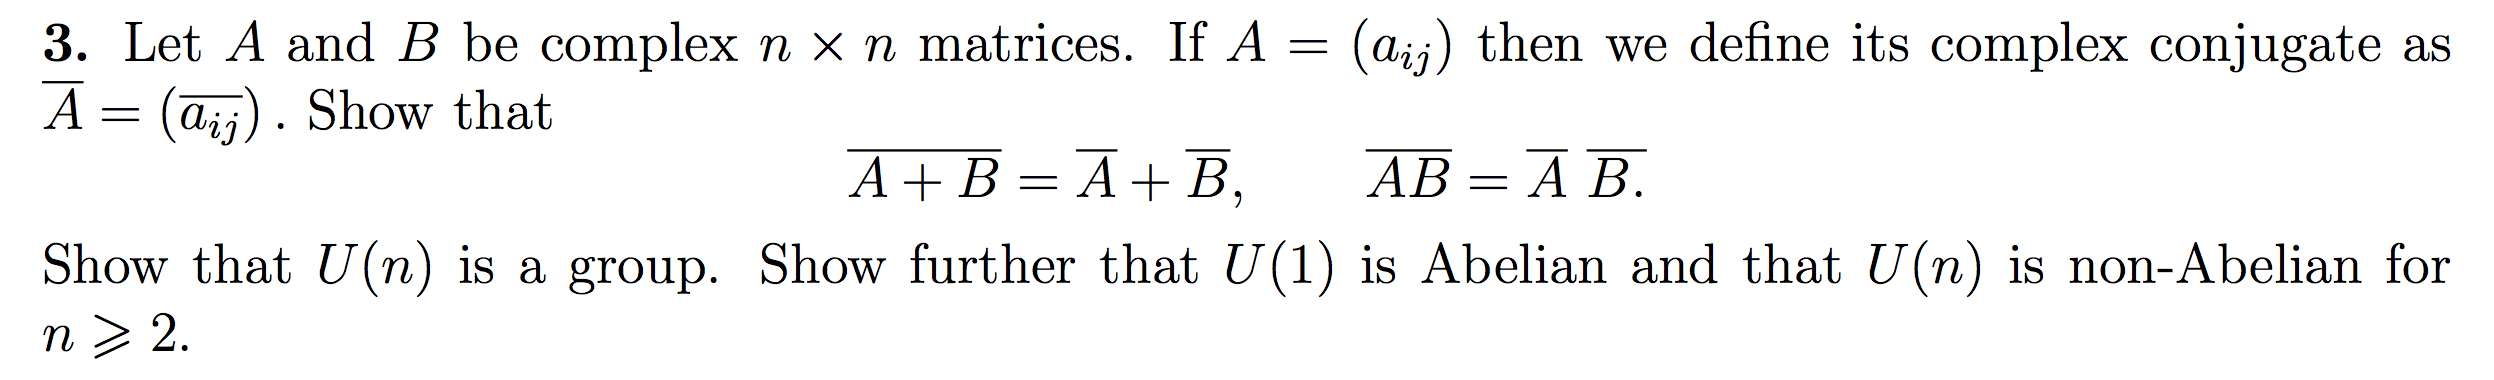
\includegraphics[width=400pt]{img/oxford-prelims-M1-groups-1-3.png}
\end{mdframed}
\begin{proof}~\\
  Let $A, B \in M_n(\C)$ be complex $n \times n$ matrices.

  It is geometrically plausible that complex conjugation preserves addition, but to confirm that:
  let $z_1 = u_1 + v_1i$ and $z_2 = u_2 + v_2i$ be complex numbers. Then
  \begin{align*}
  \bar{z_1} + \bar{z_2} = (u_1 - v_1i) + (u_2 - v_2i) = (u_1 + u_2) - (v_1 + v_2)i = \bar{z_1 + z_2}.
  \end{align*}

  For addition of complex matrices we have
  $\(\bar{A + B}\)_{ij} = \bar{a_{ij} + b_{ij}} = \bar{a_{ij}} + \bar{b_{ij}}$, proving that
  $\bar{A + B} = \bar{A} + \bar{B}$.

  For complex multiplication we have
  \begin{align*}
  \bar{z_1z_2}
    &= \bar{(u_1u_2 - v_1v_2) + (u_1v2 + v_1u_2)i}
    &=      (u_1u_2 - v_1v_2) - (u_1v2 + v_1u_2)i\\
    \text{and}\\
    \bar{z_1}~\bar{z_2}
    &= (u_1 - v_1i)(u_2 - v_2i)
    &= (u_1u_2 - v_1v_2) - (u_1v2 + v_1u_2)i,
  \end{align*}
  so $\bar{z_1z_2} = \bar{z_1}~\bar{z_2}$.

  Therefore for multiplication of complex matrices we have
  \begin{align*}
    \(\bar{AB}\)_{ij}
    = \bar{\sum_k A_{ik}B_{kj}}
    = \sum_k \bar{A_{ik}B_{kj}}
    = \sum_k \bar{A_{ik}}~\bar{B_{kj}}
    = \(\bar{A}~\bar{B}\)_{ij},
  \end{align*}
  proving that $\bar{AB} = \bar{A}~\bar{B}$.
\end{proof}

\begin{definition*}
  Let $A$ be a $n\times n$ matrix. If $A^\1 = \bar{A}^T$ then $A$ is \emph{unitary}.
\end{definition*}

\begin{proof}
  Let $U(n)$ be the set of unitary $n\times n$ matrices, under matrix multiplication.

  The identity is $I$, and inverses exist by definition of unitary.

  Associativity is inherited from the set $M_n(\C)$ of $n \times n$ matrices.

  It remains to show closure. Let $A, B$ be unitary matrices. Then
  \begin{align*}
    (AB)(\bar{AB})^T
    = (AB)(\bar{A}~\bar{B})^T
    = AB\bar{B}^T\bar{A}^T
    = AI\bar{A}^T
    = I,
  \end{align*}
  so $AB$ is indeed unitary.
\end{proof}

\begin{claim*}
  $U(1)$ is abelian.
\end{claim*}

\begin{proof}
  $U(1) \seq \C$, therefore $U(1)$ inherits commutativity from the field $\C$.
\end{proof}

\begin{claim*}
  $U(n)$ is non-abelian for $n \geq 2$.
\end{claim*}

\begin{proof}Let $O_n$ be the set of orthogonal real $n \times n$ matrices. We show that for all
  $n \geq 2$, a pair of matrices $A, B \in O_n$ exist for which $AB \neq BA$. Since
  $O_n \subset U_n$ this proves that $U_n$ is non-abelian for $n \geq 2$.

  Let $n \geq 2$ and let $\{e_1, e_2, \ldots, e_n\}$ be the standard basis for $R^n$.

  \red{TODO: correct way to talk about reflections and rotations in $n$-dimensions}

  Let $f_A:\R^n\to\R^n$ be a reflection across the subspace spanned by $\{e_2, e_3, \ldots, e_n\}$,
  so that its matrix is $A = [-e_1, e_2, e_3, \ldots, e_n]$.

  Let $f_B:\R^n\to\R^n$ be a rotation of the plane spanned by $\{e_1, e_2\}$, so that its matrix is
  $B = [e_2, -e_1, e_3, \ldots, e_n]$.

  Note that $A$ is diagonal and $A^\1 = A$, hence $A$ is orthogonal.

  Note that $B^T = [-e_2, e_1, e_3, \ldots, e_n]$ and hence $BB^T = [e_1, e_2, e_3, \ldots, e_n]$,
  hence $B$ is orthogonal.

  We have $BA = [-e_2, -e_1, e_3, \ldots, e_n] \neq AB = [e_2, e_1, e_3, \ldots, e_n]$, proving
  that $O_n$ is non-abelian for all $n \geq 2$.

  Therefore $U_n \supset O_n$ is non-abelian for all $n \geq 2$.
\end{proof}
\newpage
\begin{mdframed}
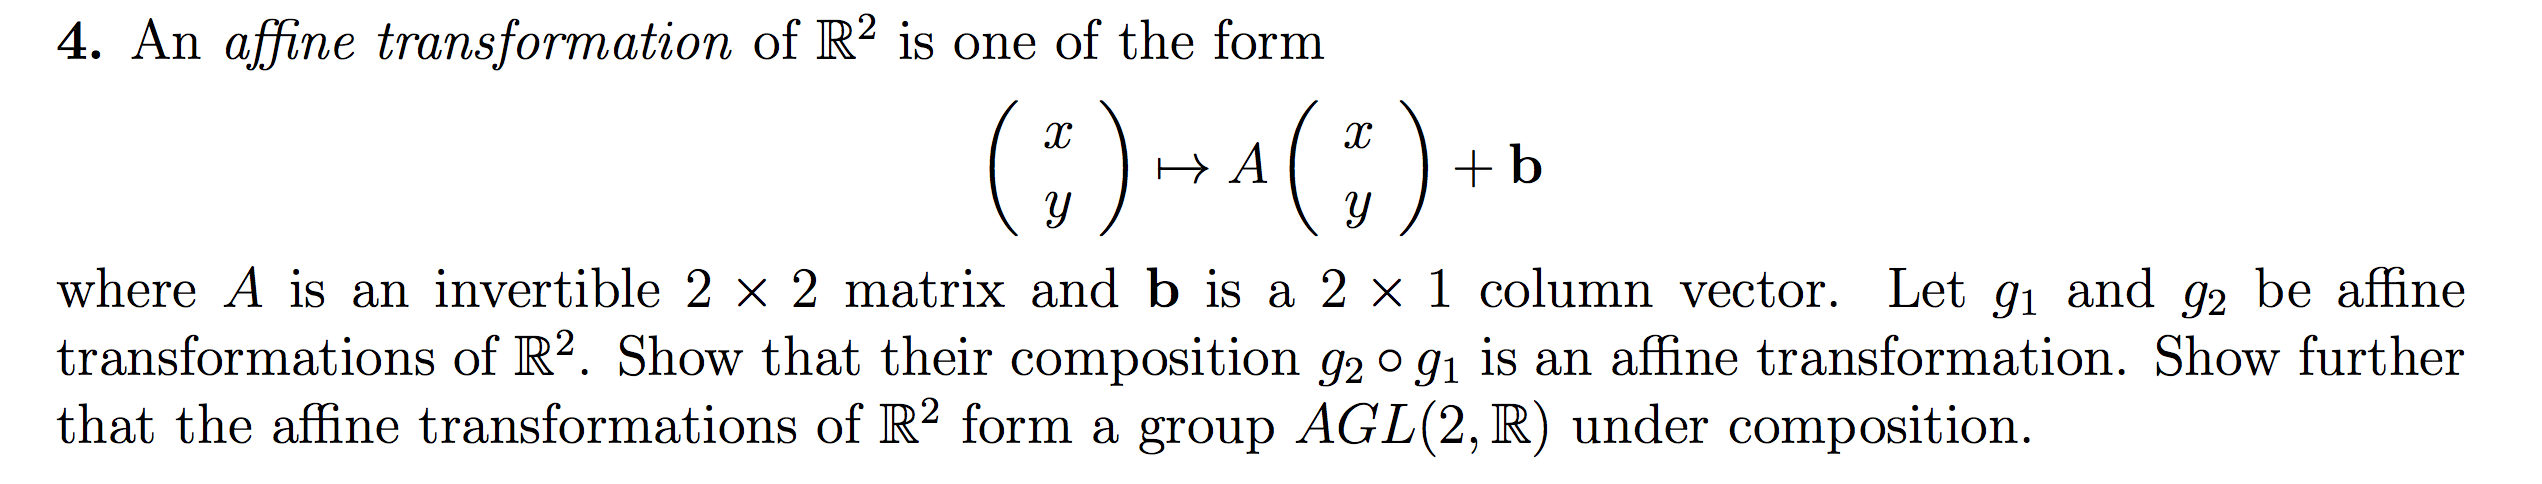
\includegraphics[width=400pt]{img/oxford-prelims-M1-groups-1-4.png}
\end{mdframed}

Let $v \in \R^2$. We have
\begin{align*}
  (g_2 \circ g_1)(v)
  = g_2(g_1(v))
  = g_2(Av + b)
  = A(Av + b) + b
  = A^2v + Ab + b,
\end{align*}
which is an affine transformation.

We have shown closure.

The group identity is the identity transformation, which is affine.

Inverses exist: let $f$ be the affine transformation given by $v \mapsto Av + b$. Then $f^\1$ is
given by $v \mapsto A^\1(v - b)$, since
\begin{align*}
(f^\1f)(v) = A^\1((Av + b) - b) = v,
\end{align*}
and
\begin{align*}
(ff^\1)(v) = A(A^\1(v - b)) + b = v.
\end{align*}

\red{We need to show associativity}.

\newpage
\begin{mdframed}
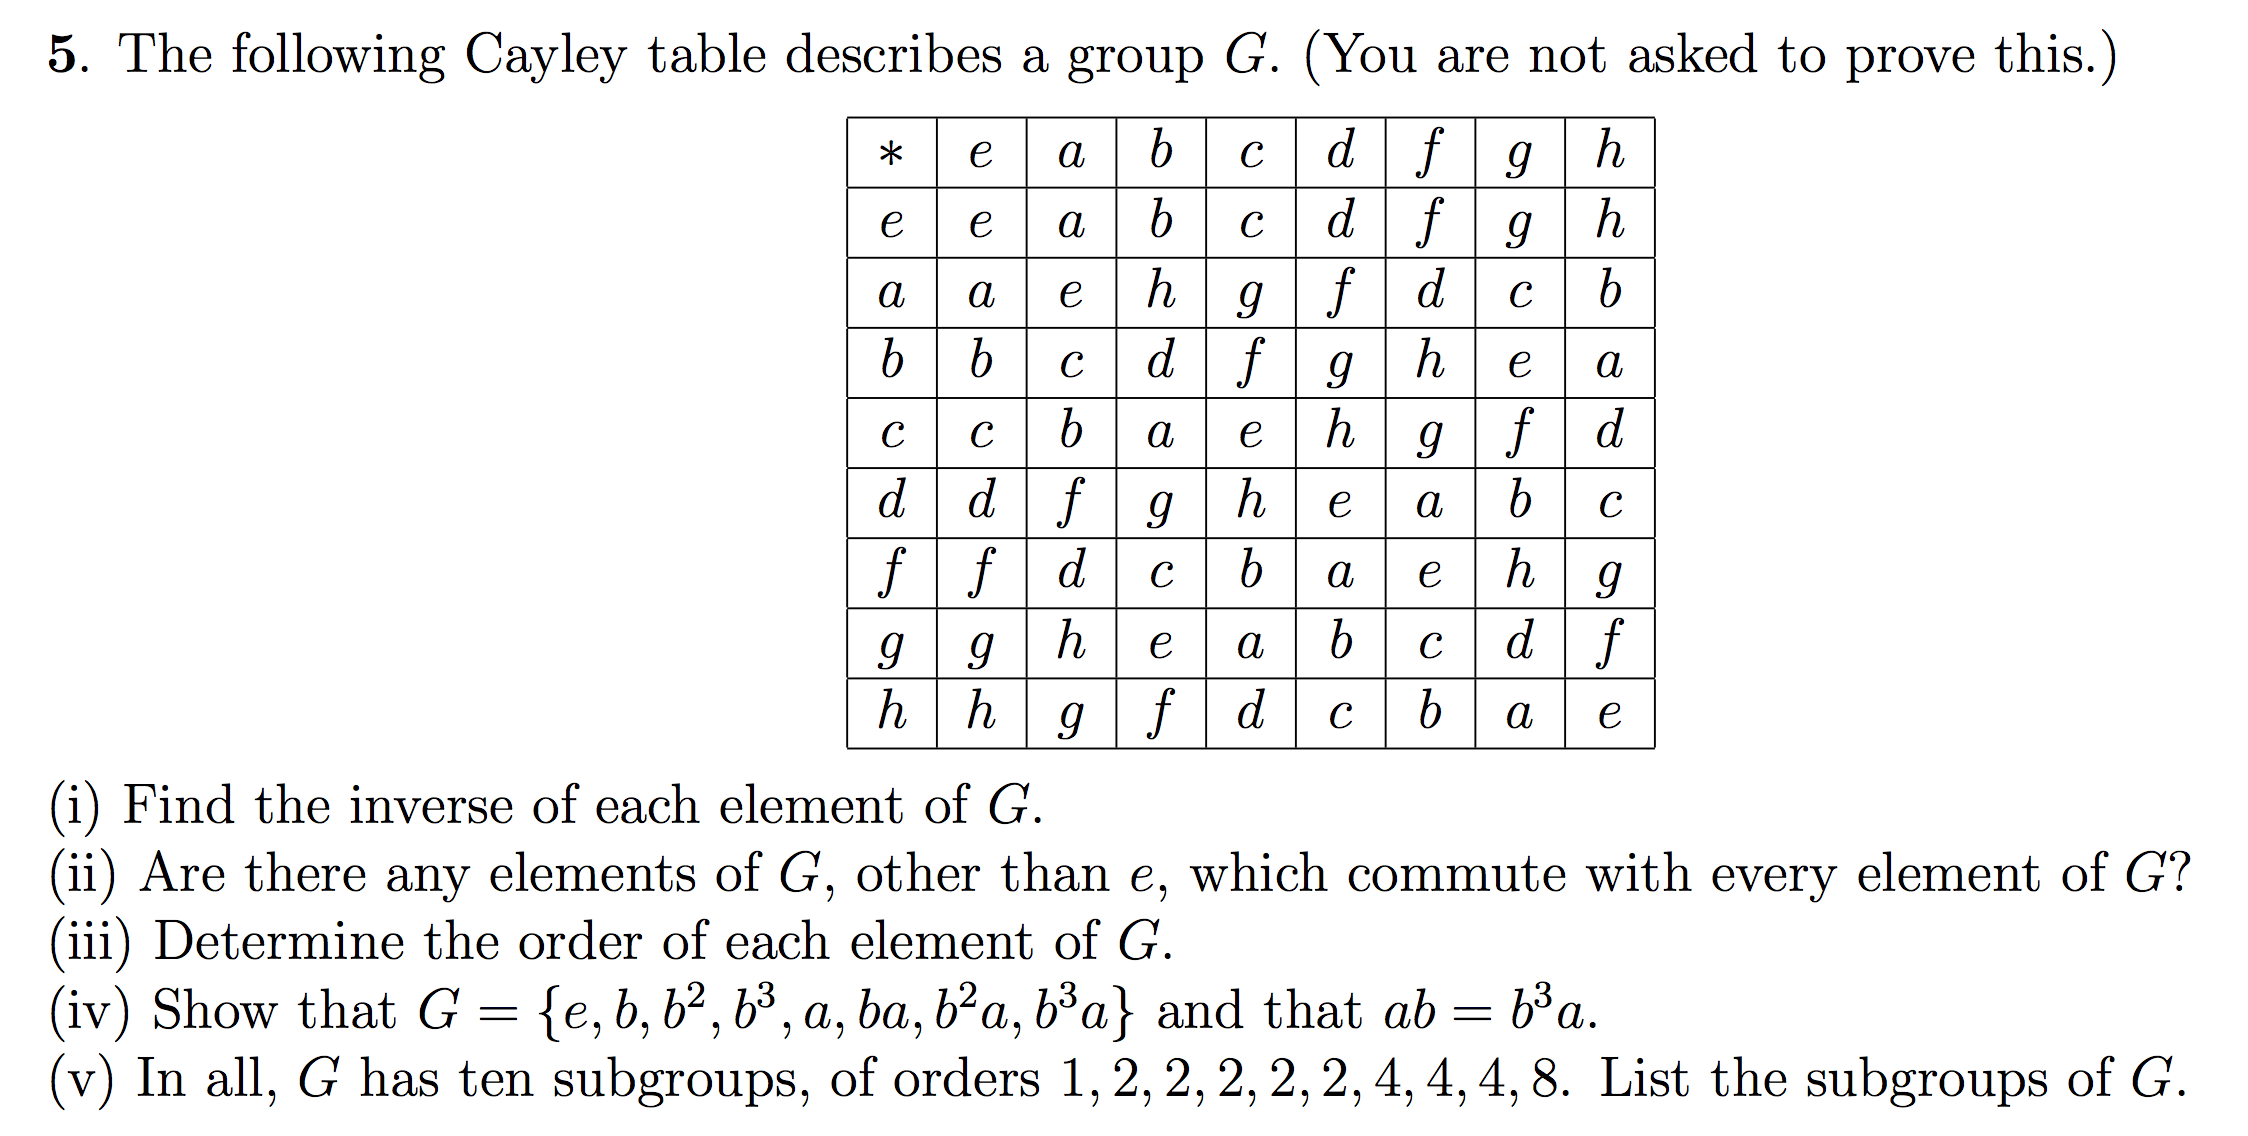
\includegraphics[width=400pt]{img/oxford-prelims-M1-groups-1-5.png}
\end{mdframed}
\begin{enumerate}[label=(\roman*)]
\item $e^\1 = e, a^\1 = a, b^\1 = g, c^\1 = c, d^\1 = d, f^\1 = f, g^\1 = b, h^\1 = h$
\item
  order of $e$ is 1\\
  order of $a$ is 2 since $a^2 = e$\\
  order of $b$ is 4 since $b^4 = d^2 = e$
\item
\end{enumerate}
\newpage
\begin{mdframed}
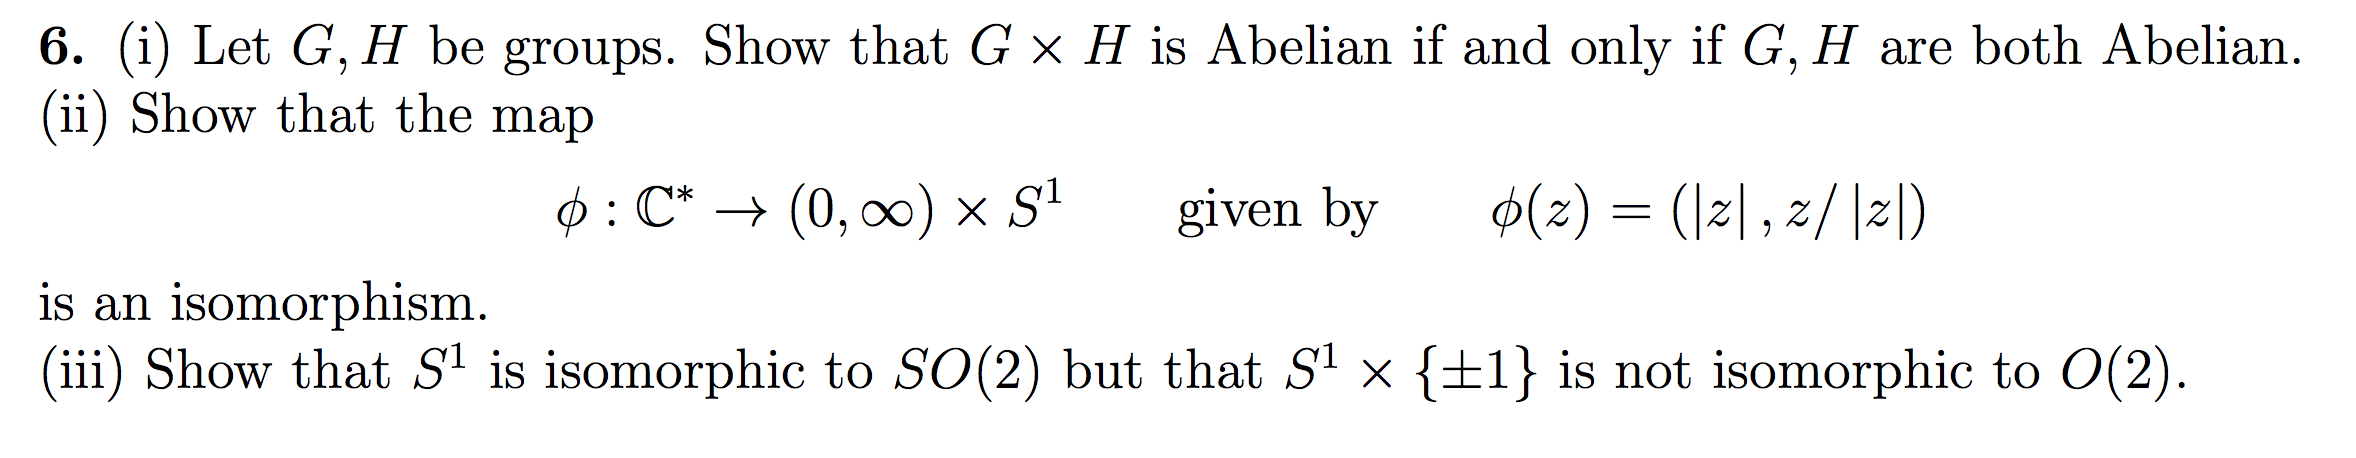
\includegraphics[width=400pt]{img/oxford-prelims-M1-groups-1-6.png}
\end{mdframed}
\begin{definition*}
  Let $G, H$ be groups. $G \times H$ is a group under the following operation:
  $(g_1, h_1) \cdot (g_2, h_2) = (g_1g_2, h_1h_2)$.
\end{definition*}

\begin{enumerate}
\item
  \begin{proof}
    Let $G, H$ be Abelian groups. Then in $G \times H$, we have
    $(g_1, h_1) \cdot (g_2, h_2) = (g_1g_2, h_1h_2) = (g_2g_1, h_2h_1) = (g_2, h_2) \cdot (g_1,
    h_1)$, so $G \times H$ is Abelian.

    Conversely, let $G \times H$ be Abelian. Then
    $(g_1, h_1) \cdot (g_2, h_2) = (g_2, h_2) \cdot (g_1, h_1)$. Therefore
    $(g_1g_2, h_1h_2) = (g_2g_1, h_2h_1)$, therefore both $G$ and $H$ are Abelian.
  \end{proof}
\item
  \begin{proof}
    To show that $\phi$ is an isomorphism, we must show that $\phi$ is injective, surjective, and
    that it preserves multiplication.

    \textbf{Injective:} Let $z_1, z_2 \in \C^*$. Suppose $\phi(z_1) = \phi(z_2) = (r,
    \theta)$. Then $|z_1| = |z_2|$ and $z_1/|z_1| = z_2/|z_2|$. Therefore $z_1 = z_2$.

    \textbf{Surjective:} Suppose there exists $(r, \theta) \in (0, \infty) \times S^1$ that is not
    in the image of $\phi$. But $\phi(r\cos\theta + r\sin\theta i) = (r, \theta)$, so no such
    $(r, \theta)$ exists.
  \end{proof}


\end{enumerate}


\newpage
\section{Sheet 5: Homomorphisms. Conjugacy. Normal Subgroups.}

\begin{mdframed}
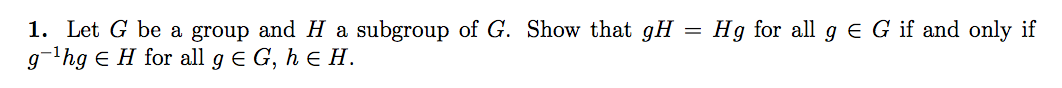
\includegraphics[width=400pt]{img/abstract-algebra-oxford-M1-5-1.png}
\end{mdframed}

\begin{claim*}
[Forwards implication]
  If $g^\1hg \in H$ for all $g \in G, h \in H$ then $gH = Hg$.
\end{claim*}

\begin{proof} We show that $Hg \subseteq gH$ and $gH \subseteq Hg$, for all $g \in G$.\\

Multiplying on the left by $g$ gives $hg \in gH$ for all $g \in G, h \in H$. Therefore $Hg \subseteq gH$ for all $g \in G$.
\end{proof}

\begin{mdframed}
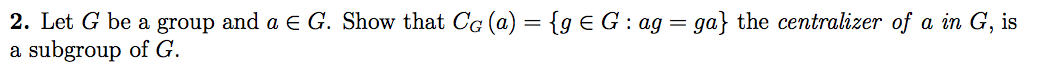
\includegraphics[width=400pt]{img/abstract-algebra-oxford-M1-5-2-1.png}
\end{mdframed}

\begin{mdframed}
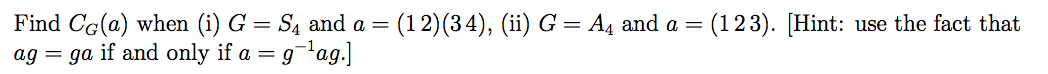
\includegraphics[width=400pt]{img/abstract-algebra-oxford-M1-5-2-2.png}
\end{mdframed}

\begin{mdframed}
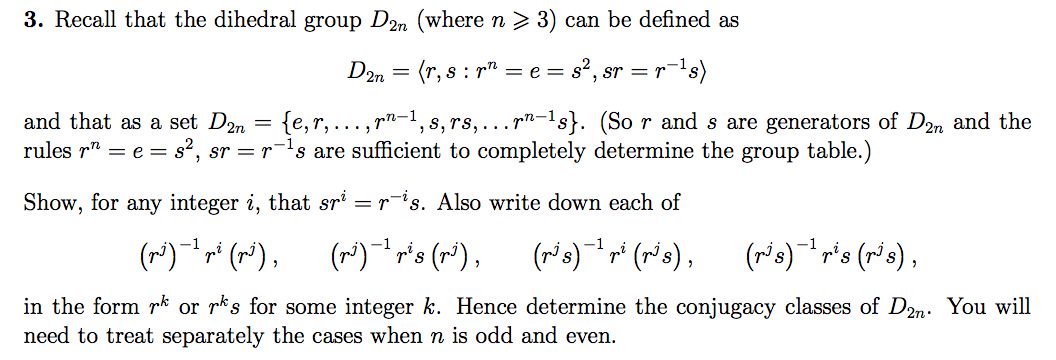
\includegraphics[width=400pt]{img/abstract-algebra-oxford-M1-5-3.png}
\end{mdframed}

\newpage
\section{Sheet 6: Quotient Groups. Isomorphism Theorem. Group Actions.}

\begin{mdframed}
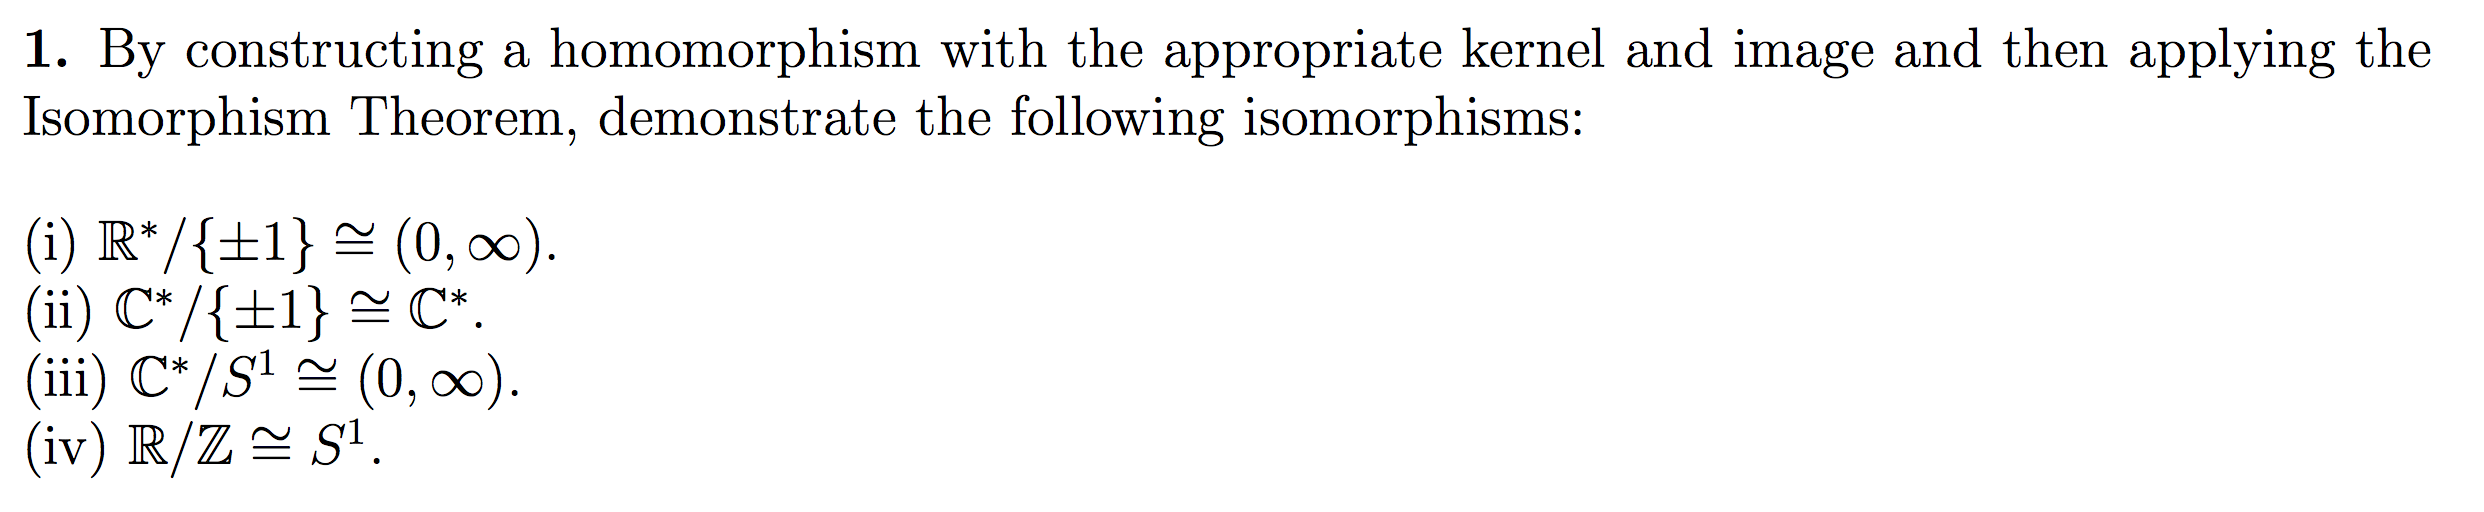
\includegraphics[width=400pt]{img/abstract-algebra-oxford-M1-6-1.png}
\end{mdframed}

\begin{theorem*}[First Isomorphism Theorem]~\\
  Let $\varphi:G_1 \to G_2$ and let $H$ be the kernel of $\varphi$. Then
  \begin{enumerate}
  \item $\Im \varphi \cong G/ \ker \varphi$
  \end{enumerate}
\end{theorem*}

\subsection*{(i): $\R^*/\{\pm 1\} \cong (0, \infty)$}

We have a group $G = \R^* = \R\setminus\{0\}$.

We have a subgroup $H = \{\pm 1\}$.

The group is abelian hence the subgroup is normal.

The set of cosets is $G/H = \{(0, \infty), (-\infty, 0)\}$.

Define the homomorphism $\varphi: G \to G/H$.

The image of $\varphi$ is the set of cosets $G/H$.

The kernel of $\varphi$ is $(0, \infty)$.

\end{document}
